% Prelim, Chapter 3
% by Rachel Slaybaugh

\chapter{Eigenvalue Acceleration}
\label{sec:Chp3}
Nuclear engineers are often concerned with finding the criticality state of a reactor. The term critical means that the fission chain reaction is self-sustaining, i.e.\ every neutron produces one new neutron. In the context of Equation~\eqref{eq:neutron transport}, this corresponds to $k = 1$. If $k < 1$, the reaction is subcritical and the total number of neutrons decreases over time. If $k > 1$, the reaction is supercritical and the total number of neutrons increases over time \cite{Duderstadt1976}. Steady-state reactor behavior is generally the operation mode of interest, and the typical concern is only the dominant eigenmode. The remaining eigenvalues can describe regional instabilities and may be useful for some analysis goals \cite{Vidal1998}. 

The ability to quickly and accurately determine the state of a multiplying nuclear system is very important in new designs. The standard eigenvalue solution methods can be slow for some cases of interest. To design new reactors, a better solver is needed. This chapter discusses the eigenvalue solver that has been implemented in Denovo to meet this challenge. Some background about eigenvalue solution methods is presented first. These methods are then put into the context of what has been done in the past and are used to explain how the added eigensolver works and why it is novel. Finally, some limited results are presented.

%-----------------------------------------------------------------------------------------
\section{Background}
Details about eigenvalue problems, characteristics of convergence, and eigenvalue solution methods are all needed to understand the eigenvalue solver that was added. The generalized eigenvalue problem takes the form $\ve{B}x = \mu \ve{C}x$ and can be transformed into an ordinary eigenvalue problem, $\ve{A}x = \lambda x$. Both forms have the same right eigenvectors. If $\ve{C}$ is non-singular then $\ve{A} = \ve{C}^{-1}\ve{B}$ and the problem $v = \ve{A}x$ can be solved in two steps: \cite{Stewart2001}
%
\begin{enumerate}
  \item $w = \ve{B}x$
  \item Solve the system $\ve{C}v = w$.
\end{enumerate}
%
Because the generalized form can be converted to the ordinary form, the formulas in this Background section will be shown in the ordinary form without loss of applicability.

Some basic notation will be needed: let $\sigma(\ve{A}) \equiv \{\lambda \in \mathbb{C} : rank(\ve{A} - \lambda \ve{I}) \le n\}$ be the spectrum of $\ve{A}$, where the elements in the set are the eigenvalues and $\mathbb{C}$ is the set of complex numbers. The eigenvalues can be characterized as the $n$ roots of the polynomial $p_{\ve{A}}(\lambda) \equiv det(\lambda \ve{I} - \ve{A})$. Each distinct eigenvalue in $\sigma(\ve{A})$ has a corresponding nonzero vector $x$ such that $\ve{A}x_{i} = \lambda_{i} x_{i}$ for $i = 1,...,n$ \cite{Sorensen1996}. It will be assumed that the eigenvalues are ordered as $|\lambda_{1}| > |\lambda_{2}| \ge \dots \ge |\lambda_{n}| \ge 0$. 

Eigenvalue problems in the nuclear transport community are typically solved with iterative rather than direct methods. A variety of iterative solvers have been used to solve eigenvalue problems. This subsection will cover the methods that have been most widely used in the nuclear field as well as methods that will aid in understanding the work being proposed. 

%-----------------------------------------------------------------------------------------
\subsection{Convergence Concerns}
Before the methods are discussed, some terms that are used to characterize how numerical methods might behave when solving problems of interest are presented. A method's behavior can be affected by characteristics of the mathematical problem ($f : X \to Y$) as well as by characterisitics of the algorithm itself ($\tilde f : X \to Y$). Most material in this section is derived from Trefethen and Bau \cite{Trefethen1997}; see this reference for more detail.

Conditioning is one way to express the perturbation behavior of the mathematical problem. A \emph{well-conditioned} problem is one in which all small perturbations of $x$ lead to only small changes in $f(x)$. An \emph{ill-conditioned} problem is one in which some small perturbation of $x$ leads to a large change in $f(x)$. The condition number is a quantity used to express how well-conditioned a matrix or problem is. A small condition number corresponds to a well-conditioned problem, and vice versa. 

The relative condition number is used to measure the effect of relative perturbations. This is particularly useful in numerical analysis because computers introduce relative errors. Let $\delta x$ be a small perturbation of $x$ and $\delta f = f(x + \delta x) - f(x)$. With these terms, the relative condition number for some norm $p$ is defined as
%
\begin{equation}
  \kappa(x)_{p} = \lim_{\delta \rightarrow 0} \sup_{||\delta x||_{p} \le \delta} \biggl(\frac{||\delta f||_{p}}{||f(x)||_{p}} / \frac{||\delta x||_{p}}{||x||_{p}} \biggr)  \:,
  \label{eq:cond}
\end{equation}
%
where $\sup$ is the supremum, the smallest real number that is greater than or equal to every number in the set in question \cite{Wikipedia2011}. This definition holds for any norm. The norm subscript will excluded unless specifying a certain norm is pertinent.

The condition number of a matrix $\mathbf{A}$ is defined as
%
\begin{equation}
  \kappa(\mathbf{A}) = ||\mathbf{A}|| \text{ }||\mathbf{A}^{-1}|| \:.
  \label{eq:condA}
\end{equation}
%
For an $n \times m$ matrix $\ve{A}$, the singular values are ordered such that $\sigma_{1} \ge \sigma_{2} \ge \dots \ge \sigma_{n} > 0$. If the two-norm is used, then $||\mathbf{A}||_{2} = \sigma_{1}$, $||\mathbf{A}^{-1}||_{2} = \frac{1}{\sigma_{m}}$, and $\kappa_{2}(\mathbf{A}) = \frac{\sigma_{1}}{\sigma_{m}}$; $\sigma_{m}$ is the $m$th singular value of $\ve{A}$. If $\mathbf{A}$ is singular, its condition number is infinity. 
%The ratio $\frac{\sigma_{1}}{\sigma_{m}}$ can be interpreted as the eccentricity of the hyper-ellipse that is the image of an $m$-dimensional unit sphere under $\mathbf{A}$. When $\ve{A}$ has a large condition number the largest principle semiaxis is much longer than the smallest principle semiaxis. 

Stability is a way to express the perturbation behavior of an algorithm used to solve a problem on a computer. %A stable algorithm ``gives nearly the right answer to nearly the right question'' \cite{Trefethen1997}. An algorithm $\tilde f$ for a problem $f$ is stable if each $x \in X$ satisfies
%\begin{equation}
%  \frac{||\tilde f(x) - f(\tilde x)||}{||f(\tilde x)||} = O(\epsilon_{machine}) \qquad \text{for some } \tilde{x} \text{ with } \frac{||\tilde x - x||}{||x||} = O(\epsilon_{machine}) \:.
%  \label{eq:stable}
%\end{equation}
%
%Backwards stability has a tighter requirement than stability alone, and a 
A backwards-stable algorithm will ``give exactly the right answer to nearly the right question'' \cite{Trefethen1997}. An algorithm $\tilde{f}$ for a problem $f$ is backwards stable if, for each $x \in X$,
%
\begin{equation}
  \tilde{f}(x) = f(\tilde{x}) \qquad \text{for some } \tilde{x} \text{ with } \frac{||\tilde{x} - x||}{||x||} = O(\epsilon _{machine}) \:.
  \label{eq:back stable}
\end{equation}

The concepts of condition and stability are not independent of one another. The accuracy of a backwards stable algorithm depends on the condition number, $\kappa(x)$ of $f$. The relative errors of an algorithm applied to some problem satisfy:
%
\begin{equation}
  \frac{||\tilde{f}(x) - f(x)||}{||f(x)||} = O(\kappa(x) \epsilon _{machine}) \:.
\end{equation}
These ideas and definitions will be needed when considering the behavior of the added eigenvalue solver in combination with the multigroup Krylov solver. 

%-----------------------------------------------------------------------------------------
\subsection{Power Iteration}
Power iteration (PI) is an old and straightforward algorithm for finding an eigenvalue/vector pair. The basic idea is that any nonzero vector can be written as a linear combination of the eigenvectors of $\ve{A}$ because the eigenvectors are linearly independent, namely $v_0 = \gamma_1 x_1 + \gamma_2 x_2 + \cdots + \gamma_n x_n$ where $x_{j}$ is the $j$th eigenvector and $\gamma_{j}$ is some constant. This specific expression assumes a non-defective $\ve{A}$, though this assumption is not necessary for the method to work. 

Another fact that is used to understand power iteration is that $\ve{A}^k x_i = \lambda_i^k x_i$. Thus
%
\begin{equation}
  \ve{A}^k v_{0} = \gamma_1 \lambda_1^k x_1 + \gamma_2 \lambda_2^k x_2 + \cdots + \gamma_n \lambda_n^k x_n \:.
  \label{eq:Ak}
\end{equation}
%
Since $|\lambda_1| > |\lambda_i|, i \ne 1$, the first term in the expansion will dominate as $k \to \infty$ and $\ve{A}^k v_{0}$ therefore becomes an increasingly accurate approximation to $x_1$. In practice, it is desirable to avoid exponentiating a matrix and it is helpful to normalize $v$ in order to avoid possible over or underflow. This leads to Algorithm \ref{algo:PI} \cite{Stewart2001}, \cite{Trefethen1997}. 
%
\begin{algorithm}
  Given $\ve{A}$ and $v_0$, $v = \frac{v_{0}}{||v_{0}||}$. \\
  Until convergence do:
  \begin{list}{}{\hspace{2em}}
    \item $w = \ve{A}v$
    \item $v = \frac{w}{||w||}$
    \item $\lambda = v^{T}\ve{A}v$
  \end{list}
  \caption{Power Iteration}
  \label{algo:PI}
\end{algorithm}

Using Equation \eqref{eq:Ak} and Algorithm \ref{algo:PI}, PI's convergence behavior can be understood. After $k$ steps, the iteration vector will be: 
%
\begin{equation}
  v_{k} = \bigl( \frac{\lambda_{1}^{k}}{e_{1}^{T}\ve{A}^{k}v_{0}} \bigr) \bigl(\frac{1}{\lambda_{1}^{k}}\ve{A}^{k}v_{0} \bigr) \:.
\end{equation}
% 
If $\ve{A}$ has eigenpairs $\{(x_{j}, \lambda_{j}), 1 \le j \le n \}$ and $v_{0}$ has the expansion $v_{0} = \sum_{j=1}^{n} x_{j}\gamma_{j}$ then
%
\begin{equation}
  \frac{1}{\lambda_{1}^{k}}\ve{A}^{k}v_{0} =  \frac{1}{\lambda_{1}^{k}} \sum_{j=1}^{n} \ve{A}^{k}x_{j}\gamma_{j} = \sum_{j=1}^{n} x_{j} \bigl(\frac{\lambda_{j}}{\lambda_{1}} \bigr) \gamma_{j} \:.
  \label{eq:PIexpand}
\end{equation}
%
From equation \eqref{eq:PIexpand} it can be determined that the error is reduced in each iteration by a factor of $|\frac{\lambda_{2}}{\lambda_{1}}|$, which is called the dominance ratio. If $\lambda_2$ is close to $\lambda_1$, then this ratio will be close to unity and the method will converge very slowly. If $\lambda_2$ is far from $\lambda_1$, then convergence will happen much more quickly. Put simply, PI is better suited for problems where $\ve{A}$ has eigenvalues that are well separated \cite{Sorensen1996}.  

Power iteration is very attractive because it only requires matrix-vector products and two vectors of storage space. Because of its simplicity and low storage cost, PI has been widely used in the transport community for criticality problems for quite some time \cite{Lewis1993}, \cite{Warsa2004a}. Despite these beneficial characteristics many current codes use an acceleration method with PI, or have moved away from it altogether because of the slow convergence for many problems of interest. Nevertheless it is still used in some codes, has historical relevance, and is used in many studies as a base comparison case. 

As an aside, it is interesting to point out the connection between Krylov methods and power iteration. The power method is a Krylov method that uses a subspace of dimension one.  A Krylov subspace is built by storing the vectors created during each iteration of the power method. Krylov methods with subspaces larger than one take advantage of the information generated during each iteration that the power method discards. 

%-----------------------------------------------------------------------------------------
\subsection{Shifted Inverse Iteration}
One way to improve power iteration is to shift the matrix $\ve{A}$ and then, in a power iteration-type scheme, apply the inverse of the shifted matrix rather than the regular unshifted matrix. The method is called inverse iteration or shifted inverse iteration and the goal is to provide better convergence properties. Understanding why shifted inverse iteration is an improvement requires understanding spectral transformation. 

The fundamental notion is that $\ve{A}$ can be shifted by a scalar without changing the eigenvectors. That is, for some shift $\mu$, $(\ve{A} - \mu \ve{I})$ will have the same eigenvectors as $\ve{A}$ \cite{Sorensen1996}. If $\mu \notin \sigma(\ve{A})$, then $(\ve{A} - \mu \ve{I})$ is invertible and $\sigma([\ve{A} - \mu \ve{I}]^{-1}) = \{1/(\lambda - \mu):\lambda \in \sigma(\ve{A})\}$. Eigenvalues of $\ve{A}$ that are near the shift will be transformed to extremal eigenvalues that are well separated from the others. Such a spectral transformation can be added to the power method. Given an estimate, $\mu \approx \lambda_1$, the shifted inverse power method will usually converge more quickly than PI.

To see why this works consider: 
%
\begin{equation}
    \tau_1 = \frac{1}{\lambda_1 - \mu}\text{ , }\tau_2 = \frac{1}{\lambda_2 - \mu}\text{ , }\dots\text{ , }\tau_n = \frac{1}{\lambda_n - \mu} \:.
\end{equation}
%
As $\mu \to \lambda_1$, $\tau_1 \to \infty$ and all the other eigenvalues go to finite quantities. If the $\tau$s are inserted into the convergence analysis done for PI, it can be shown that the shifted inverse power method will reduce error in every iteration by a factor of $\frac{|\lambda_{1} - \mu|}{|\lambda_{2} - \mu|}$. This is typically much faster than $|\frac{\lambda_{2}}{\lambda_{1}}|$, though the ultimate success of the method is dependent upon the quality of the shift \cite{Sorensen1996}, \cite{Trefethen1997}. 

The algorithm for shifted inverse iteration is much like that for power iteration, requiring only one change. Step 1 becomes ``solve $(\ve{A}-\mu \ve{I})w = v$;'' all other steps are the same. After convergence, the actual eigenvalue of interest is backed out using the eigenvector \cite{Sorensen1996}.  Shifted inverse iteration is effectively the same as performing power iteration on $(\ve{A}-\mu \ve{I})^{-1}$. 

On initial consideration it would seem shifted inverse methods might not work well when the shift is very good because the matrix becomes very ill-conditioned. If the shift is exact, i.e.\ when $\mu = \lambda_{1}$, the matrix is singular. It turns out this concern is unfounded. Peters and Wilkinson proved that ill-conditioning is not a problem for inverse iteration methods \cite{Peters1979}. Trefethen and Bau also assert that this is the case as long as the $(\ve{A}-\mu \ve{I})w = v$ portion is solved with a backwards stable algorithm \cite{Trefethen1997}.

Wielandt's method is a flavor of shifted inverse iteration that has been used widely in the neutron transport community, though it was originally developed in 1944 in an unrelated context \cite{Zinzani2008}, \cite{Itagaki1996}, \cite{Itagaki2002}, \cite{Ipsen}. In the transport equation formulation, Wielandt's method changes the generalized form of the eigenvalue problem to $(\ve{I} - \ve{DL}^{-1}\ve{M}(\ve{S} +\gamma_e \ve{F}))\phi = \delta \gamma \ve{DL}^{-1}\ve{MF} \phi$ where $\gamma_e$ is an estimate for the eigenvalue $\gamma_1 = \frac{1}{k}$, $\phi$ is the corresponding eigenvector, and $\delta \gamma = \gamma_1 - \gamma_e$. The power method is applied to this, giving \cite{Nakamura1977}
%
\begin{equation}
\phi^{i+1} = \delta \gamma^{i}(\ve{I} - \ve{DL}^{-1}\ve{M}(\ve{S} + \gamma_e \ve{F}))^{-1}\ve{DL}^{-1}\ve{MF}\phi^{i} \:. \label{eq:Wielandt}
\end{equation}

The estimate, $\gamma_e$, can be improved on each iteration by starting with an initial guess of $0$ and setting $\gamma_e^i = \delta \gamma^{i-1} + \gamma_e^{i-1} + \alpha$. Here $\alpha$ is an optional small positive constant that is designed to keep roundoff error from dominating when $\gamma_e$ becomes very close to $\gamma_1$ \cite{Nakamura1977}. 

Studies of reactor systems have found shifted inverse iteration to be faster than power iteration \cite{Allen2002}. In the general computational community, shifted inverse iteration has largely taken the place of power iteration when looking for eigenvectors associated with eigenvalues that are relatively well known at the outset of the calculation since this information allows for the selection of a good shift \cite{Ipsen}.  

%-----------------------------------------------------------------------------------------
\subsection{Rayleigh Quotient Iteration}
Rayleigh quotient iteration is a variation of shifted inverse iteration that has a changing shift like Wielandt's method sometimes does. The key difference is that this method uses a specific formula, the Rayleigh quotient (RQ), that is designed to find the optimal the shift at every iteration. 

The Rayleigh quotient for the ordinary eigenvalue problem, originally proposed by the third Baron Rayleigh in the 1870s, is defined as \cite{Parlett1974}:
%
\begin{equation}
  \rho(x, \ve{A}) = \rho(x) = \frac{x^{T}\ve{A}x}{x^{T}x} \:.
  \label{RQ}
\end{equation}
%
If $x$ is an eigenvector of $\ve{A}$, then the RQ is the corresponding eigenvalue. If $x$ is close to an eigenvector, then the RQ will approximate the eigenvalue \cite{Stewart2001}. The derivation of the RQ comes from asking the question ``what $\alpha$ will minimize $||\ve{A}x - \alpha x||_2$?'' Solving this using least squares will give $\alpha = \rho(x)$ \cite{Trefethen1997}. 

The RQ has a similar form for the generalized eigenvalue problem, mentioned here because it applies to some of the past work discussed below and is the form that was implemented in the added solver. For the problem $\ve{A}x = \lambda \ve{B}x$, there is a right eigenpair $(\lambda, x)$ for $x \ne 0$ and a left eigenpair $(\lambda, y): y^{T}\ve{A} = \lambda y^{T}\ve{B}$ for $y \ne 0$. Let $\langle \alpha, \beta \rangle$ be a simple eigenvalue of pencil $(\ve{A}, \ve{B})$. If $x$ and $y$ are right and left eigenvectors corresponding to $\langle \alpha, \beta \rangle$, respectively, then $\langle \alpha, \beta \rangle = \langle y^{T} \ve{A} x, y^{T} \ve{B} x \rangle$. This means the ordinary form of the eigenvalue is:
\begin{equation}
 \lambda = \frac{y^{T} \ve{A} x}{y^{T} \ve{B} x} \:,
\end{equation}
which is the generalization of the RQ \cite{Stewart2001}. 

Recall from the previous section that choosing a shift close to the eigenvalue of interest controls the dominance ratio of shifted inverse iteration, and hence convergence behavior. The RQI algorithm uses a strategically selected shift, the Rayleigh quotient, as seen in Algorithm \ref{algo:RQI} \cite{Trefethen1997}, \cite{Parlett1974}.
\begin{algorithm}
  Given $\ve{A}$ and $v_{0}$, $v = \frac{v_{0}}{||v_{0}||}$, and $\rho_{0} = \rho(v) = v^{T}\ve{A}v$ \\
  Until convergence do:
  \begin{list}{}{\hspace{2.5em}}
    \item Solve $(\ve{A} - \rho\ve{I})w = v$
    \item normalize $v = \frac{w}{||w||}$
    \item form $\rho = v^{T}\ve{A}v$
  \end{list}
  \caption{Rayleigh Quotient Iteration}
  \label{algo:RQI}
\end{algorithm}
%
This process generates a sequence, $\{\rho_{k}, v_{k}\}$, called the Rayleigh sequence generated by $v_{0}$ on $\ve{A}$. To more deeply understand why this method is optimal and useful for the purposes of this work, more properties of the Rayleigh quotient are highlighted \cite{Parlett1974}: 
%
\begin{itemize}
  \item For $\alpha \ne 0$, $\rho(\alpha x, \ve{A}) = \rho(x, \ve{A})$, so using any multiple of $x$ will produce the same sequence as $x$. 
  \item The RQ has translational invariance, $\rho(x, \ve{A} - \alpha \ve{I}) = \rho(x,\ve{A}) - \alpha$, meaning the matrix $(\ve{A} - \alpha \ve{I})$ produces the same sequence as $\ve{A}$ \cite{Parlett1974}. This relationship can be used to relate eigenvalues and applied shifts. In fact, this is one of the ways to find the eigenvalue of interest for the standard shifted inverse iteration method \cite{Sorensen1996}. 
\item When $x$ is an eigenvector of $\ve{A}$, $\rho(x)$ is stationary at $x$.  
\item When $x \ne 0$ the RQ gives the minimal residual, with equivalence holding only when $\beta = \rho(x)$:
%
\begin{equation}
  ||(\ve{A} - \beta\ve{I})x||^{2} \ge ||\ve{A}x||^{2} - ||\rho(x)x||^{2} \:.
\end{equation}
%
\item $x$ is orthogonal to $(\ve{A} - \rho(x))x$. 
\end{itemize}

RQI has very good convergence properties for normal matrices. The minimal residual property of the RQ causes the global convergence behavior. The sequence of residuals $\{ ||(\ve{A} - \rho_{k})v_{k}|| = ||r_{k}||, k = 0, 1, ... \}$ is monotonically decreasing for all starting $v_{0}$. When RQI is applied to normal matrices, the following has been proven as $k \to \infty$:
%
\begin{enumerate}
 \item $\rho_{k} = \rho(v_{k})$ converges, and either
 \item $(\rho_{k}, v_{k})$ converges cubically to an eigenpair $(\lambda, k)$, or
 \item $\rho_{k}$ converges linearly to a point equidistant from $s \ge 2$ eigenvalues of $\ve{A}$, and the sequence $\{v_{k}\}$ cannot converge. 
\end{enumerate}
%
This means that when RQI converges to the correct eigenpair it does so rapidly. However, there is a risk that if a bad starting vector is selected it will not converge at all \cite{Parlett1974}. 

The monotone sequence $\{||r_{k}||\}$ is bounded from below by 0. If the limit of the sequence is 0 as $k \to \infty$ then case 2 will be observed and convergence will be cubic. If the limit is greater than 0, case 3 is found. Unfortunately, it does not seem that this can be know \emph{a priori}. In practice, however, users found that it was difficult to make the method fail for normal matrices \cite{Parlett1974}. 

For non-normal matrices the stationary property does not hold, which means the convergence is quadratic at best. The residual sequence is also not guaranteed to be monotonically decreasing and thus no global convergence properties can be proven. It has been found in practice that RQI will still converge for non-normal systems, just at a slower rate than for normal matrices. However, convergence cannot be guaranteed nor predicted in advance \cite{Parlett1974}. 

%To deal with this, two adapted RQI methods for non-normal matrices were developed that attempt rectify this. One developed Ostrowski regains the stationary property at eigenvectors. In the non-defective case this gives cubic convergence, but gives no guarantees of global convergence. The other was developed by Parlett and it generates monotonically decreasing residuals, thus guaranteeing global convergence but at a rate that is merely linear for non-defective matrices \cite{Parlett1974}. 

%-----------------------------------------------------------------------------------------
\subsection{Krylov Methods}
The multigroup Krylov solver is used over all energy groups inside RQI in Denovo. Because this requires applying a Krylov method to a shifted system, some additional facts about Krylov methods are needed. Krylov subspaces have the property that for any $\mu$, $\mathcal{K}_k(\ve{A}- \mu \ve{I}, x) = \mathcal{K}_k(\ve{A},x)$. This means that a Krylov method can be applied to a shifted system and the correct eigenvector will still be found \cite{Stewart2001}. 

Convergence and stability properties differ from Krylov method to Krylov method. Because GMRES is the most widely used Krylov method in this work, convergence and stability discussions will focus on this method. Regarding stability, Paige et.\ at.\  \cite{Paige2006} demonstrate that the least squares solution at every step in GMRES is always backwards stable. 

GMRES is also backwards stable when finding $x$ in $\ve{A}x = b$ for ``sufficiently nonsingluar $\ve{A}$.'' An $n \times n$ $\ve{A}$ that qualifies as nonsingular enough satisfies
%
\begin{equation}
  \ve{A}x = b \ne 0\:, \qquad \ve{A} \in \mathbb{R}^{n \times n} \:, \qquad b\in \mathbb{R}^{n} \:, \qquad \sigma_{min}(\ve{A}) \gg n^{2}\epsilon ||\ve{A}||_{F} \:.
\end{equation}
%
Here $\epsilon$ is the floating point arithmetic unit roundoff, $|| \cdot ||_{F}$ is the Frobenius norm, and $\sigma_{min}(\ve{A})$ is the minimum singular value of $\ve{A}$. Using the notation that $\ve{\tilde V}_{m}$ is the $n \times m$ orthonormal matrix computed at step $m$ of the modified Gram-Schmidt procedure during the Arnoldi process and includes rounding error, GMRES is also backwards stable up until  \cite{Paige2006}
%
\begin{equation}
  \kappa_{2}(\ve{\tilde V}_{m}) = \frac{\sigma_{max}(\ve{\tilde V}_{m})}{\sigma_{min}(\ve{\tilde V}_{m})} \le \frac{4}{3} \:.
\end{equation}

To analyze convergence, Trefethen and Bau \cite{Trefethen1997} point out that evaluating GMRES is facilitated by relating it to a polynomial approximation problem. GMRES solves this approximation problem: find $p_{n} \in P_{n}$ such that 
%
\begin{align}
  ||p_{n}(\ve{A})b||_{2} &= \text{minimum,} \qquad \text{where}  \nonumber \\
  P_{n} &= \{ \text{polynomials } p \text{ of degree } \le n \text{ with } p(0)=1 \nonumber \}.
\end{align}
%
This polynomial requires the first coefficient to be 1, which is a normalization at $z=0$ . GMRES chooses the coefficients of the polynomial $p_{n}$ to minimize the norm of the residual, $r_{n} = b - \ve{A}x_{n} = (\ve{I} - \ve{A}q_{n} (\ve{A}) )b$; $q_{n}$ is a polynomial of degree $n-1$ and $p_{n}(z) = 1 - zq(z)$ \cite{Trefethen1997}.

GMRES is monotonically convergent: $||r_{n+1}||_{2} \le ||r_{n}||_{2}$. In addition, $||r_{n}||_{2} = ||p_{n}(\ve{A})b||_{2} \le ||p_{n}(\ve{A})||_{2}$ $||b||_{2}$. Thus, the convergence rate of GMRES is determined by
%
\begin{equation}
  \frac{||r_{n}||_{2}}{||b||_{2}} \le \inf_{p_{n}\in P_{n}} ||p_{n}(\ve{A})||_{2} \:.
\end{equation}
%
To get an idea of how quickly GMRES can converge, the question of how small $||p_{n}(\ve{A})||_{2}$ can be for a given $n$ and $\ve{A}$ must be answered. For this analysis let $\ve{A}$ be diagonalizable such that $\ve{A}=\ve{X} \Lambda \ve{X}^{-1}$, where $\Lambda = \Lambda(\ve{A})$ is a diagonal matrix of eigenvalues for $\ve{A}$ and $\ve{X}$ is a non-singular matrix of eigenvectors. Also define the scalar $||p||_{S} = \sup_{z\in S} |p(z)|$. Then \cite{Trefethen1997}
%
\begin{equation}
  ||p(\ve{A})||_{2} \le ||\ve{X}||_{2} \text{ } ||p(\Lambda)||_{2} \text{ } ||\ve{X}^{-1}||_{2} = \kappa_{2}(\ve{X}) ||p||_{\Lambda(\ve{A})} \:.
\end{equation}

All of this can be combined to say that at step $n$ of GMRES, the residual satisfies
%
\begin{equation}
  \frac{||r_{n}||_{2}}{||b||_{2}} \le \kappa_{2}(\ve{X})  \inf_{p_{n}\in P_{n}} ||p||_{\Lambda(\ve{A})} \:.
  \label{eq:GMRES normal bound}
\end{equation}
%
This means that the convergence of GMRES depends on how far $\ve{A}$ is from normal and how quickly the size of $p_{n}(\ve{A})$ on the spectrum $\Lambda(\ve{A})$ decreases with $n$ \cite{Trefethen1997}. 

Nachtigal et.\ al.\ \cite{Nachtigal1992} derive a similar bound for any arbitrary $\ve{A}$, removing the diagonalizable assumption. In this case let $\Lambda_{\epsilon} \supseteq \Lambda$ be the $\epsilon$-pseudospectrum of $\ve{A}$. The set of pseudo-eigenvalues are the points $z \in \mathbb{C}$ that are eigenvalues of some matrix $\ve{A} + \ve{E}$ with $||\ve{E}|| \le \epsilon$ and $\epsilon > 0$. Let $L$ be the arclength of the boundary $\partial \Lambda_{\epsilon}$. Then
%
\begin{equation}
  \frac{||r_{n}||_{2}}{||b||_{2}} \le \frac{L}{2 \pi \epsilon} \inf_{p_{n}\in P_{n}} ||p||_{\Lambda_{\epsilon}(\ve{A})} \:.
  \label{eq:GMRES arbitrary bound}
\end{equation}
%
For an arbitrary $\ve{A}$, the convergence of GMRES depends on the polynomial approximation defined on the pseudospectrum rather than the spectrum. The implications of the relationships in Equations \eqref{eq:GMRES arbitrary bound} and \eqref{eq:GMRES normal bound} are, however, similar.

While these assertions are for GMRES, the experience of the computational community indicates the conclusions extend to most Krylov methods. For ill-conditioned systems Krylov methods may not be backwards stable and tend to converge very slowly. As a result, many researchers have found that Krylov methods must be preconditioned to be able to get good results in practice \cite{Benzi2002}, \cite{Trefethen1997} , \cite{Paige2006}. 

%-----------------------------------------------------------------------------------------
%-----------------------------------------------------------------------------------------
\section{Past Work}
The ideas from the previous section will provide meaning and significance for past related work as well as for the new work. %This section will be restricted to eigenvalue methods used for solving neutronics problems, i.e.\ the neutron diffusion and transport equations. Some methods are intended to find multiple eigenpairs rather than just the dominant eigenmode. While multiple eigenmodes are not of interest here, the methods developed in this work could be easily extended to handle such cases if desired. 
There are three main areas of past work that are pertinent to the added method. The first is an overview of how others have and do solve the eigenvalue neutron diffusion and transport problems. The next is Denovo's current eigenvalue solution method. The third is what happens when Krylov methods are applied to ill-conditioned systems.

\subsection{Eigenvalue Solution Methods}
A review of the literature leads to a variety of useful observations that will be discussed: shifted inverse iteration (SII) is generally better than power iteration; the key to succeeding with SII is selecting a good shift; there are a variety of eigenvalue solution methods used in diffusion and transport; and no one has used RQI to solve the transport equation.

It has been common practice to use the power method to solve both the diffusion and transport eigenvalue equations. However, it is well known that PI converges very slowly for systems with loosely coupled or optically thick fission regions and thus SII is often pursued as an alternative choice. For many problems SII converges more rapidly than PI \cite{Adams2002}, \cite{Evans2011}. Allen and Berry compared the power method and the shifted inverse power method for the one-group, one-dimensional transport equation and found that the inverse method converges much more quickly \cite{Allen2002}. 

Itagaki used Wielandt's spectral shift technique to solve the one-group, 3-D diffusion equation for various problem types, including systems containing strong neutron absorption. Itagaki's numerical results illustrate some problems with this method. When the estimate $\lambda_e$ is not good, the correct eigenvalue may never be found \cite{Itagaki1996}, \cite{Itagaki2002}. 

An analysis of the Ringhals reactor was done using two-group, finite difference diffusion with Wielandt's method. When doing actual core analysis it was found that the local flux shape around the control rods made the flux converge slowly. The only way to improve convergence was to use a good initial guess for the flux \cite{Hotta1997}. 

Quite recently Zinzani et.\ al.\ modified the Wielandt method for the two-group diffusion equation to be able to find multiple eigenmodes. The method removes the requirement of a good initial guess, making it more robust than Wielandt's original method. %This group formulates the problem as $\ve{C}\phi = \frac{1}{k}\ve{F}\phi \Rightarrow \ve{C}^{-1}\ve{F}\phi_{n} = k_{n}\phi_{n}$, where the iteration index is $n$. To affect the action of $\ve{Y} = \ve{C}^{-1}\ve{F}$ they first multiply by $\ve{F}$ and then apply $\ve{C}^{-1}$ using a direct method. Zinzani et.\ al.\ use approximate minimum degree ordering to reorder $\ve{C}$. They then use LU factorization to find the dominant eigenvector. The shift is applied in the process of finding the eigenvalue. 
%
%To find the next eigenvector they remove the fission contribution coming from the just found mode, and do power iteration to find the next mode\cite{Zinzani2008}. This is called the elimination method \cite{Modak2006}. 
Numerical results showed their method to be accurate and robust, but the algorithm is complicated and quite slow \cite{Zinzani2008}.%. They also used an explicitly restarted Arnoldi method which they found to be much faster than their modified power method

These studies demonstrate, as is expected given the theoretical considerations discussed above, that shifted inverse iteration performs better than power iteration for many problems, and the degree to which it is better often depends upon the quality of the shift and the initial guess for the eigenvector.

Eigenvalue solution methods that are not based on power iteration have started to become prevalent in the last 20 years. Many of these methods use Krylov subspace methods, and some use the Rayleigh quotient in various ways. 

In 1988 Suetomi and Sekimoto used a Rayleigh Quotient Minimization (RQM) method to solve the one-group, 2-D diffusion equation in the form of a generalized $k$-eigenvalue problem. This method is a minimization problem for the Rayleigh quotient; the minimal RQ gives the best eigenvalue and corresponding eigenvector estimate. The monoenergetic diffusion equation is symmetric positive definite (SPD), so incomplete factorization preconditioned CG was used to find the minimum RQ. The preconditioned RQM method performed better than both unpreconditioned RQM and power iteration with SOR as the inner iteration solver \cite{Suetomi1988}. 

In 1991 Suetomi and Sekimoto extended their work to the few-group, 2-D, $k$-eigenvalue diffusion problem. This system is no longer SPD and as a result they could not use CG. Instead they chose a conjugate residual method called ORTHOMIN(1). This functions like CG, but has a slightly different formulation and cannot use the Rayleigh quotient. The ORHTOMIN(1) method requires that the symmetric portions of the matrices be positive definite. They again used incomplete factorizations for preconditioning and compared the method with PI, finding results similar to the one-group case \cite{Suetomi1991}.  

In 2004 Gupta and Modak used Suetomi and Sekimoto's work as a basis for a method to solve the generalized eigenvalue form of the transport equation. The group noted ORTHOMIN(1) could be applied to the transport equation in the same way that Suetomi and Sekimoto applied it to the diffusion equation. This method would solve the entire problem at once, removing the inner-outer iteration structure. However, Gupta and Modak elected not to pursue this approach because it required the explicit formation of both the transport and fission matrices. For 3-D, multigroup transport problems, forming and storing these matrices can be quite expensive. In addition, rewriting transport solvers to handle the implementation would be difficult \cite{Gupta2004}.
 
To overcome these obstacles, Gupta and Modak changed the original method such that it retained the inner-outer structure and did not require explicit matrix formation. This approach made the problem smaller and only required the ability to solve a fixed-source problem. They used TSA accelerated SI in the inner iterations to find group fluxes, and ORTHOMIN(1) was applied as the outer iteration method. The new method was compared to the power method using SI and TSA accelerated SI. In two test problems they found ORHTOMIN(1) with TSA to be faster than PI \cite{Gupta2004}. 

Beginning in 1997 Vidal, Verd\'u, and others began a development stream in which they solved the multigroup, downscattering only, $k$-eigenvalue diffusion equation with both the Implicitly Restarted Arnoldi Method (IRAM) and another subspace method that is a generalization of the power method \cite{Vidal1997}, \cite{Vidal1998}, \cite{Verdu1999}. 

Vidal et.\ al.\ used Rayleigh-Ritz projection and symmetric Rayleigh-Ritz projection as subspace iteration methods to solve the downscattering only, two-group, 3-D diffusion equation using nodal collocation as the spatial discretization. The methods use block sweeps that are solved with an iterative method like CG with a Jacobi preconditioner. For each iteration they get an approximate set of eigenvectors, $\ve{X}_{n}$, orthonormalize the set to get $\ve{X}_{n+1}$, and then compute the Rayleigh-Ritz projection: $\hat{\ve{Y}}^{n+1} = (\ve{X}^{n+1})^{T} \ve{Y} \ve{X}^{n+1}$. The eigenvalue problem is then solved with $\hat{\ve{Y}}^{n+1}$ to get the new estimate for the eigenvectors \cite{Vidal1998}. 

They also developed a variational acceleration technique that takes advantage of the fact that all dominant eigenmodes in a reactor are physically real. They found the symmetric method to be better than the general method and that the acceleration technique gave some improvement \cite{Vidal1998}. In related work, Vidal et.\ al.\ compared the Rayleigh-Ritz methods with an explicitly restarted Arnoldi method, all of which have been parallelized, for the two-group diffusion equation \cite{Vidal1997}. 

Verd\'u et.\ al.\ extended Vidal et.\ al.'s 1998 work \cite{Vidal1998} to find multiple eigenvalues for the two-group diffusion equation. They compared the power method, the symmetric Rayleigh-Ritz method with variational acceleration, and an implicitly restarted Arnoldi method. The restarted Arnoldi code they chose was IRAM. Verd\'u's group slightly modified the original method for the diffusion equation. It was found that IRAM was much faster than the Rayleigh-Ritz method and both were much better than power iteration \cite{Verdu1999}. Hern\'andez et.\ al.\ applied a parallel implementation of IRAM to the two-group neutron diffusion problem \cite{Hernandez1998}.

These different approaches have largely been applied to the diffusion approximation, though a few have been extended to the transport equation. Several of the diffusion solution methods make use of the Rayleigh quotient, though none have done Rayleigh Quotient Iteration itself. Nearly all studies that used SII were only applied to a few groups. No examples where RQI was used an eigenvalue solution method for the neutron transport equation were found. 

\subsection{Denovo's Power Iteration}
Before this work, the eigenvalue solution method used by Denovo was similar to what is done in other 3-D transport codes. Recall the operator form of the transport equation seen in Equation \eqref{eq:operator-form}. This equation can be combined with $\phi = \mathbf{D} \psi$ and manipulated in the following ways:
%
\begin{equation}
  \phi = \ve{DL}^{-1}\ve{MS}\phi + \ve{DL}^{-1}\ve{M}\frac{1}{k}\ve{\chi} \ve{f}^{T} \phi \:.
\end{equation}
%
Let $\ve{T} = \ve{DL}^{-1}$, rearrange, and multiply both sides by $f^{T}$:
  %
\begin{align}
  f^{T}\bigl(\ve{I} - \ve{TMS}\bigr)\phi &= \frac{f^{T}}{k} \ve{TM}\chi f^{T} \phi \:, \label{eq:OperatorEvalForm} \\
  %
  \text{define } \Gamma &= f^{T}\phi  \text{ and rearrange} \:, \nonumber \\
  %
  k \Gamma &= \underbrace{f^{T}(\ve{I} - \ve{TMS})^{-1} \ve{TM} \chi}_{\ve{A}} \Gamma \:. \label{eq:OrdinaryEigenvalue}
\end{align}
%
All of that can be used to make the traditional form of power iteration where the eigenvalue iteration index is $k$:
%
\begin{equation}
  \Gamma^{k+1} =  \frac{1}{k^{k}}\ve{A} \Gamma^{k} \:.
\label{eq:PowerItForm} 
\end{equation}
Note that Equation~\eqref{eq:OrdinaryEigenvalue} is the ordinary form of the eigenvalue transport equation. In this case the eigenvalue-vector pair are $(\Gamma, k)$. 

The application of $\ve{A}$ to $\Gamma^{k}$ involves a multigroup solve that looks like a fixed source problem:
%
\begin{equation}
  \bigl(\ve{I} - \ve{TMS}\bigr)y^{k} = \ve{TM}\chi \Gamma^{k} \:.
\end{equation}
%
This means outer iterations update the eigenvalue and there are two sets of inner iterations: energy, and space-angle, just like other fixed source solves. Originally, a Krylov solver was used for the space-angle inner iterations and Gauss Seidel was used for the energy iterations \cite{Evans2009a}, \cite{Evans2011}. Denovo uses Trilinos \cite{Heroux2003} to provide the Krylov solver, with a choice of either GMRES or BiCGSTAB \cite{Evans2009}.

\subsection{Concerns with Krylov Methods}
As has been mentioned, Krylov methods have frequently been applied to the solution of the transport equation. It has often been found that these Krylov methods do not converge well when they are not preconditioned. The first observation of unsatisfactory behavior was by Lewis in 1977 when CG was applied to the 1-D, symmetrised, $S_{N}$ transport equation. The formulation used had a large condition number and that likely caused the problem \cite{Lewis1977}, \cite{Gupta2004}. 

Recent work in 1- and 2-D transport analysis has highlighted that restarted GMRES can stagnate in problems with optically thin subdomains \cite{Rosa2010}. In 1998 Oliveira and Deng studied the application of a variety of Krylov methods to the 1-D neutron transport equation. They found that all of these methods can converge slowly for problems of interest if they are not preconditioned \cite{Oliveira1998}. The recognition that Krylov methods can have convergence problems in transport calculations led Patton and Holloway to study how different preconditioners improve the performance of GMRES when applied to the 1-D, $S_{N}$ transport equation. They focused on GMRES because they found it to be faster and less memory intensive than other Krylov methods \cite{Patton2002}. 

These experiences emphasize that Krylov methods can have serious convergence problems in practice. These methods particularly have trouble with poorly conditioned problems and cases with optically thin regions, which are cases of interest in real transport calculations.  

%-----------------------------------------------------------------------------------------
%-----------------------------------------------------------------------------------------
\section{RQI in Denovo}
A better eigenvalue solution method is needed to be able to do cutting edge, high-fidelity calculations. The last two sections illustrated that a shifted inverse iteration method could provide substantial benefit over power iteration, particularly if an optimal shift is chosen. This observation inspired the addition of Rayleigh Quotient Iteration as an eigenvalue solver in Denovo. The balance of this chapter will cover the details of the method implementation, present some results, and discuss the implications of RQI.

%-----------------------------------------------------------------------------------------
\subsection{Method}
To implement RQI in Denovo, the shift was applied in a manner similar to Wielandt's method. To see how this works, subtract $\rho \ve{TMF}$ from both sides of $(\ve{I} - \ve{TMS})\phi = \lambda \ve{TMF}\phi$, where $\rho$ is the Rayleigh quotient and $\lambda = \frac{1}{k}$. This gives the following shifted system:
%
\begin{align}
  [\ve{I} - \ve{TM}(\ve{S} + \rho\ve{F})]\phi &=( \lambda - \rho) \ve{TMF} \phi \:. \\
  \text{ Now define } \ve{\tilde{S}} &\equiv \ve{S} + \rho\ve{F} \text{ to write} \nonumber \\
   [\ve{I} - \ve{TM\tilde{S}}]\phi &=( \lambda - \rho) \ve{TMF} \phi \:.
    \label{eq:OperatorShiftedEval}
\end{align}

The scattering matrix is lower triangular for groups that have downscattering. There are entries above the diagonal only when there is upscattering. The fission matrix has an energy-block filled column for every group with fission. Applying the shift as $(\ve{S} + \rho \ve{F})$ makes the scattering matrix energy-block dense even when there is very little upscattering. Thus, the new matrix, $\ve{\tilde{S}}$, is energy-block dense and looks like one big upscattering block.

A key element that enabled the choice of RQI is the multigroup Krylov solver. Traditional solution methods for the fixed source part of the equation, like Gauss Seidel, do not handle energy-block dense scattering matrices well. This has hampered the implementation of SII in multi-group, 3-D codes because solving many groups that have upper-triangular scattering entries will take a long time. Because RQI uses the MG Krylov solver, it can also take advantage of the associated energy decomposition. 

The energy-parallelized RQI method is shown in Algorithm \ref{algo:RQI+MGkrylov}. Here $\ve{A} = [\ve{I} - \ve{TMS}]$ and a block of energy groups corresponding to an energy set is denoted by superscript ${\tilde{g}}$. The moments being computed by a given energy set are indicated by $\phi^{\tilde{g}}$.
%
\begin{algorithm}[!h]
  Break the problem into energy sets and distribute to the appropriate number of processors\\
  Get initial guesses for $\phi$ and set $k_{old} = k_{0}$\\
  Calculate the initial Rayleigh quotient, $\rho_{old}$, using Algorithm \ref{algo:calcRQ}\\
  Until convergence:
  \begin{list}{}{\hspace{2.5em}}
     \item Calculate the right shift: $\mu = \frac{1}{k_{old}} - \rho_{old}$
     \item Shift both sides by 
     \begin{enumerate}
       \item subtracting $\rho_{old} [\ve{TMF}]^{\tilde{g}}$ from $\ve{A}^{\tilde{g}}$ and 
       \item making the right hand side $\mu [\ve{TMF}]^{\tilde{g}} \phi^{\tilde{g}}$
    \end{enumerate}
    \item Use the MG Krylov solver to solve $[\ve{I} - \ve{TM\tilde{S}}]^{\tilde{g}}\phi^{\tilde{g}} = \mu [\ve{TMF}]^{\tilde{g}} \phi^{\tilde{g}}$ for an updated $\phi^{\tilde{g}}$
    \item Global barrier so all processes can finish calculating $\phi^{\tilde{g}}$; all processes get the new $\phi$
    \item $k_{old} = \frac{1}{\rho_{old}}$
    \item Calculate a new Rayleigh quotient, $\rho_{new}$; $k_{new} = \frac{1}{\rho_{new}}$
    \item Compare $k_{old}$ and $k_{new}$ for convergence 
    \item Update the iterates, $k_{old} = k_{new}$; $\rho_{old} = \rho_{new}$
  \end{list}
  \caption{Rayleigh Quotient Iteration in Denovo}
  \label{algo:RQI+MGkrylov}
\end{algorithm}
%
Denovo's implementation of RQI uses the generalized form of the Rayleigh quotient: $\frac{\phi^{T} \ve{A} \phi}{\phi^{T} \ve{TMF} \phi}$. The way this is computed using energy sets is shown in Algorithm \ref{algo:calcRQ}. 
%
\begin{algorithm}[!h]
  \begin{list}{}{\hspace{2.5em}}
    \item denominator $= \phi_{old}^{\tilde{g}, T} [\ve{TMF}]^{\tilde{g}} \phi_{old}^{\tilde{g}}$
    \item Globally sum the denominator
    \item If $|$denominator$|$ $> 1 \times 10^{-13}$, 
      \begin{list}{}{\hspace{1em}}
        \item numerator  $= \phi_{old}^{\tilde{g}, T} \ve{A}^{\tilde{g}} \phi_{old}^{\tilde{g}}$
        \item Globally sum the numerator
        \item $\rho = \frac{\text{numerator}}{\text{denominator}}$
      \end{list}
    \item Else, $\rho = \frac{1}{k_{old} + 1 \times 10^{-6}}$ 
  \end{list}
  \caption{Calculating the Rayleigh Quotient}
  \label{algo:calcRQ}
\end{algorithm}

There is also an option to simply do shifted inverse iteration instead of RQI. In this case the user chooses a fixed shift, $\beta$, that is used in place of $\rho$ when shifting the matrices. Algorithm \ref{algo:RQI+MGkrylov} can be modified to accommodate this choice by changing $\rho$ to $\beta$ in the calculation of $\mu$ and the ``Shift both sides'' step. The Rayleigh quotient is still calculated at every iteration to make the new estimate for $k$. 

The current implementation of Denovo's operator and solvers does not allow the RQI method to work with multisets when there are reflecting boundaries. This solution option combination is not necessary in this work nor in the analysis of the potential value of RQI. An important development step in the future will be to add this functionality to Denovo. A detailed explanation of the reason for the current code limitation is given in Appendix \ref{sec:AppendixC}.

%-----------------------------------------------------------------------------------------
\subsection{Results}
A few calculations were done to investigate whether RQI is an improvement over power iteration. The quality of improvement is measured by the total number of Krylov iterations rather than timing. This is a more meaningful measure because some calculations were so small and ran so fast that timing was inaccurate, this is a metric that can be compared across computers, and there may be room for some optimization in the future that would change the timing. GMRES was the Krylov method used in all cases unless noted otherwise.

Before RQI was added to Denovo, an infinite medium scoping code was written in Python to test that the algorithm worked in that very simple case.  Using this code a 4-group, a 7-group, and a 27-group problem were solved. In all cases RQI and PI both converged on the first iteration to the correct answer. 

The first Denovo problem chosen was a small, few-group system intended to demonstrate the new solver's correctness. In fact, it is a unit test built into Denovo's test suite intended to verify that all parts of the code behave correctly. This problem used a 3 $\times$ 3 $\times$ 3 grid with 0.1 spacing, vacuum boundary conditions, two materials, four groups that were only downscattering, $S_{2}$, $P_{0}$, had all tolerances set to 1 $\times$ 10$^{-6}$, a dominance ratio of 0.1396, and a reference $k$ of 0.11752. The small dominance ratio implies that PI should preform reasonably well on this problem. The debug version of Denovo was used and the calculation and was not parallelized in any way. 

This problem was solved with RQI and PI, both using the MG Krylov solver for the multigroup iterations. Note that when PI is used with MG Krylov all the downscatter groups are still solved using the forward substitution method one group at a time rather than as a block. The RQI method used MG Krylov over the whole block because of the effective upscattering added by the shift. 

\begin{table}[!h]
\caption{RQI Unit Test with Vacuum Boundaries, Power Iteration Compared to Rayleigh Quotient Iteration}
\begin{center}
\begin{tabular}{| c | c | c | c | c |}
\hline
Solvers & $k$ & Group Iters & Eigen Iters & Total Krylov \\[0.5ex]
\hline
PI &  0.11752 &  2 or 3 / group & 7 & 73 \\
RQI &  0.11752 & 4 to 8 & 6 & 39 \\
\hline
\end{tabular}
\end{center}
\label{table:SmallVacuumRQI}
\end{table}
%
The results are given in Table \ref{table:SmallVacuumRQI}. The term ``Group Iters'' either refers to the number of within-group iterations (in the case of PI) or multigroup iterations where the Krylov vector is over all groups (in the case of RQI). Both RQI and PI got the correct answer. PI used a total of 73 Krylov iterations while RQI used a total of 39 Krylov iterations. 

The subspace sizes in these two calculations are not the same, and because of the shift the matrices being applied within each Krylov solve are also different. These differences mean the cost of the two methods cannot be quantitatively compared in a precise way when considering iteration count. For this problem with all downscattering, the application of RQI is likely more costly than PI. 

Nevertheless, a few important heuristic observations can be made. RQI was able to calculate both the correct eigenvector and correct eigenvalue in a small number of iterations. And while RQI may not be better than PI for this problem with a small dominance ratio, it is at the very least not much worse. 

The second problem was nearly the same as the first, but was intended to test the reflecting boundary case. This is also a unit test. For this problem all boundaries were reflecting and only one material was used. These changes made the dominance ratio 1.630 $\times$ 10$^{-15}$ and $k$ became 2.0. These results can be seen in Table \ref{table:SmallReflectingRQI}. The conclusions that can be drawn from this test are the same as from the last, with the addition that this one demonstrates RQI works with reflecting boundaries. 
%
\begin{table}[!h]
\caption{RQI Unit Test with Reflecting Boundaries, Power Iteration Compared to Rayleigh Quotient Iteration}
\begin{center}
\begin{tabular}{| c | c | c | c | c |}
\hline
Solvers & $k$ &  Group Iters & Eigen Iters & Total Krylov \\[0.5ex]
\hline
PI & 2.0 & 9 / group & 2 & 72 \\
RQI & 2.0 & 17 and 18 & 2 & 35 \\
\hline
\end{tabular}
\end{center}
\label{table:SmallReflectingRQI}
\end{table}

This problem was also solved using the fixed shift option. A shift of 1.95 was selected, and this gave the same behavior as RQI. The fixed shift option was not extensively tested in this work. Shifted inverse iteration is a method that has been used for transport before and is therefore not of particular interest. It is simply noted here that this option exists and initial testing indicates that it works. 

The first two small tests plus the infinite medium experience show that RQI can get the right answer and that with very simple problems perform at least not much worse than power iteration. While these small successes were encouraging, they were not sufficient to demonstrate that the method is successful. 

To continue investigation, an intermediate-size problem was tried next. This system had a 9 $\times$ 9 $\times$ 9 spatial grid with 0.5 spacing, reflecting boundary conditions, one material, 27 groups, 13 upscattering groups, $S_{2}$, $P_{1}$, the overall tolerance was 1 $\times$ 10$^{-3}$, the upscattering tolerance was 1 $\times$ 10$^{-6}$, and the eigenvalue tolerance was 1 $\times$ 10$^{-5}$. The dominance ratio was 6.32 $\times$ 10$^{-13}$ and the reference $k$ was 0.4003. 

When PI with MG Krylov was used the correct answer was obtained in 2.57 $\times$ 10$^{2}$ seconds. The calculation needed 90 Krylov iterations per eigenvalue iteration and two outer iterations for a total of 180 Krylov iterations to converge. 

When RQI was used with MG Krylov, the problem did not converge. The maximum number of Krylov multigroup iterations per eigenvalue iteration was set to 1,000 and this was taken every time except the first, which took 25. That means the eigenvector was not converging. The calculation was terminated after 40 eigenvalue iterations. The value of $k$ oscillated between 0.3966 and 0.3967. While the problem did not converge, the estimated eigenvalue was close to the right value.

This test was also tried using BiCGSTAB instead of GMRES for the Krylov solver since BiCGSTAB has different convergence properties. This change did not improve things. The eigenvector exhibited the same behavior, requiring all the multigroup iterations for each eigenvalue iteration. After seven eigenvalue iterations the problem terminated because a negative eigenvalue was calculated. In Denovo a calculation terminates if a negative value for $k$ is found. Choosing to use BiCGSTAB made the results worse for this problem. 

With an even more difficult problem RQI did not even find nearly the correct eigenvalue when using GMRES. The two-dimensional C5G7 mox benchmark problem \cite{OECD-NEA2003} was selected for investigation and was solved with an optimized version of Denovo. This problem used three enrichment levels, an external mesh file, two reflecting boundaries to make it 2-D, 10 materials, 7 groups, 4 upscattering groups, $S_{2}$, $P_{0}$, an overall tolerance and upscatter tolerance of 1 $\times$ 10$^{-3}$, an eigenvalue tolerance of 1 $\times$ 10$^{-5}$, $k_{0}$ set to 1.14, and had a dominance ratio of 0.7709. The reference $k$ is 1.18655 $\pm$ 0.008.

\begin{table}[!h]
\caption{2-D C5G7 Benchmark, Power Iteration Compared to Rayleigh Quotient Iteration}
\begin{center}
\begin{tabular}{| l | c | c | c | c |}
\hline
Solvers & $k$ & MG Iters & Eigen Iters & Total Krylov \\[0.5ex]
\hline
PI + TTG GS & 1.18538 & 157 GS & 32 & 21,365 \\
PI +  MG Krylov & 1.18702 &  $\sim$100 & 32 & 3,129 \\
RQI & $\sim$0.95 & 1,000 & 120$^{*}$ & 119,006 \\
\hline
\end{tabular} \\
$^{*}$Terminated manually
\end{center}
\label{table:2DMoxRQI}
\end{table}
%
The results from this calculation are presented in Table \ref{table:2DMoxRQI}. Here power iteration was used with both accelerated Gauss Seidel (TTG GS) and with MG Krylov. PI + TTG GS needed a total of 21,365 single-group-sized Krylov iterations and PI + block Krylov needed 3,125 all-group-sized Krylov iterations to converge. Regarding the new multigroup solver, it is of interest that the PI + block Krylov calculation took slightly less time than PI + TTG GS. 

The most important result, however, was that with RQI the eigenvector did not converge and the eigenvalue was wrong. Except for the first, every set of multigroup iterations went to the maximum iteration count of 1,000. Using BiCGSTAB instead of GMRES was also tried for the 2-D problem without success. Finally, a 3-D version of the C5G7 mox benchmark problem \cite{OECD-NEA2005} was tried with RQI. This, too, did not converge.  

\begin{figure}[!ht]	
  \begin{center}
    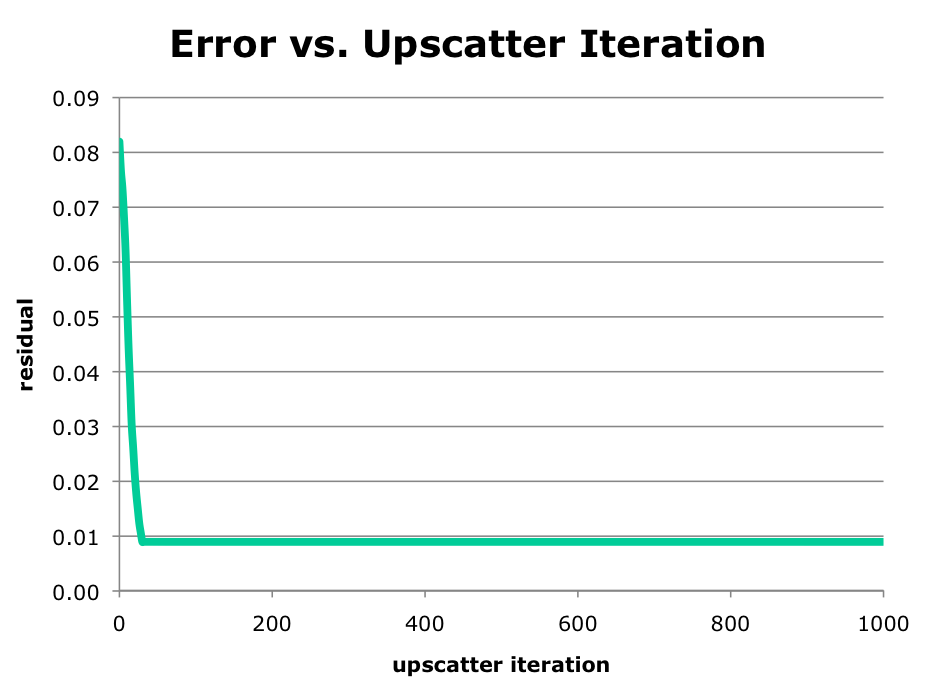
\includegraphics [width=0.75\textwidth, height=0.4\textheight ] {RQIConvergenceFail}
  \end{center}
  \caption{2-D C5G7 Benchmark, Residual as a Function of Upscatter Iteration Count for One Eigenvalue Iteration}
  \label{fig:RQIConvergenceFail}
\end{figure}
%
Figure~\ref{fig:RQIConvergenceFail} shows a plot of the residual vs. multigroup iteration count for one RQI eigenvalue iteration in the 2-D case. It is clear that error reduction stalls and the eigenvector does not converge. When the Krylov iterations do not converge, the flux estimate is not good. Without a good approximation to the eigenvector, the RQ is no longer a valid approximation to the eigenvalue and thus the eigenvalue problem does not converge. It is likely that the eigenvector does not converge because RQI creates poorly conditioned systems. Krylov methods do not handle ill-conditioned systems very well and may converge extremely slowly when trying to solve them. 

This hypothesis is supported by the fact that during the first eigenvalue iteration GMRES does converge. During this first iteration the shifts are made from an RQ computed with the initial moments and the initial $k$. The RQ is likely not close to the actual eigenvalue and the right shift is likely not close to zero. This means the system will not be too ill-conditioned. 

After the eigenvector converges on that first iteration it may be that the RQ becomes close enough to $\lambda_{1}$ that the system is ill-conditioned enough to prevent subsequent multigroup iterations from converging in the specified number of iterations. The system seems to be in a middle ground where the eigenvalue-vector pair are not good enough to converge the calculation, but are good enough to keep the system ill-conditioned. 

An additional concern is that when the system is ill-conditioned GMRES may no longer be backwards stable. If GMRES is not backward stable, then there is no guarantee that RQI will converge. It is worth noting that there is no evidence that, given a sufficient amount of computing time, RQI would converge to the wrong answer. There is certainly not data to support the claim that RQI will converge to the proper eigenvalue in all cases, but it is heartening to notice there is also not data indicating that it will not. 

Overall, though, the observed behavior strongly suggests that the multigroup Krylov method should be preconditioned so that the eigenvector will converge. If that happens it is likely that RQI will then converge as well. Only with preconditioning can the real benefit of RQI be properly investigated.

%-----------------------------------------------------------------------------------------
\subsection{Implications}
Rayleigh quotient iteration is an old method that is an adaptation of shifted inverse iteration. Because the RQ provides an optimal shift, it is expected that using RQI in Denovo will converge in fewer iterations than power iteration for some problems, provided that the eigenvector is converged. 

Further, this solver is wrapped around the MG Krylov solver from Chapter \ref{sec:Chp2}. It has already been demonstrated that the energy decomposition works and improves solution time and code scaling for fixed source multigroup problems. It is therefore reasonable to expect that when the method converges, decomposing the entire matrix in energy for eigenvalue calculations will work and provide the same kind of scaling improvement.

The intermediate and large problems that were tested demonstrate that RQI does not converge for even slightly challenging problems. This is probably caused by the poor condition number created by RQI. When the multigroup Krylov solver is not preconditioned it cannot converge the eigenvector in many cases. The incorrect eigenvector subsequently creates an incorrect eigenvalue. 

The small problems showed that RQI can get the correct solution and that the number of iterations is comparable to PI for very simple problems. For difficult problems RQI could be beneficial if the multigroup iterations can be converged. If the MG Krylov solver is preconditioned, then it may be able to converge the eigenvector for cases of interest. To really investigate the benefit of RQI, a good preconditioner is needed. The work in the next chapter is tied to this issue.

RQI has not been applied to the transport equation before because it takes $O(n^{3})$ operations for full dense matrices, and without parallelization in energy it could be prohibitively expensive \cite{Stewart2001}. In the past, adding a shift to make the scattering matrix energy-block dense was difficult to handle. The system would have been solved with Gauss Seidel, which would have been restrictively slow. The multigroup Krylov algorithm has enabled energy parallelization and made it possible to calculate the eigenvector with a shifted system.

Computers that facilitate enough parallelization to decompose in energy and have enough memory to store Krylov subspaces for the full transport equation make combining RQI and MG Krylov possible. The resulting convergence of the eigenvalue should be faster than PI for at least some problems. The energy decomposition will allow eigenvalue calculations to overcome the limitations of KBA and be scaled to many more cores. These ideas have never before been used together in this way. 

\separatorpage{}
